\section{Repetitive steps in compilers development}
In Section \ref{sec:introduction} we briefly stated that the process of developing a compiler includes several steps that are repetitive, i.e. their behaviour is always the same regardless of the language for which the compiler is built. In this section we show in what way this process is repetitive and what is the common pattern 

\subsection{Type checking}
Type systems are generally expressed in the form of logical rules \cite{cardelli1996type}, made of a set of premises, that must be verified in order to assign to the language construct the type defined in the conclusion. For example the following rule defines the typing of an \texttt{if-then-else} statement in a functional programming language:\footnote{Note that the type rule of \texttt{if-then-else} in an imperative programming language is different.}

\begin{mathpar}
	\mprset{flushleft}
	\inferrule*{\Gamma \vdash c : bool \quad \Gamma \vdash t : \tau \quad \Gamma \vdash e : \tau}
	{\Gamma \vdash \text{if \textit{c} then \textit{t} else \textit{e}} : \tau}
\end{mathpar}

\noindent
In this rule $\Gamma$ is the environment. The type rule first evaluates the premises, which means that if the condition of the \texttt{if-then-else} has type \texttt{bool} and both \texttt{then} and \texttt{else} blocks have the same type, then the whole \texttt{if-then-else} has the type of either blocks.

Typing a construct of the language requires to evaluate its corresponding typing rule. In order to do so, the behaviour of each typing rule must be implemented in the host language in which the compiler is defined. Independently of the chosen language, the behaviour will always be the following : (\textit{i}) evaluate a premise, (\textit{ii}) if the evaluation of the premise fails then the construct fails the type check and an error is returned, (\textit{iii}) repeat step 1 and 2 until all the premises have been evaluated, and (\textit{iv}) assign the type to the construct that is defined in the rule conclusion.

\subsection{Semantics}
Semantics define how the language abstractions behave and can be expressed in different ways, for example with a term-rewriting system \cite{klop1992term} or with the operational semantics \cite{plotkin1981}. For the scope of this work, we choose to rely on the operational semantics. The definition of the operational semantics of a language abstraction is, again, in the form of a logical rule where the conclusion (which is the final behaviour of the construct) is achieved if the evaluation of the premises lead to the desired results. For instance, the operational semantics of a while loop could be the following:

\begin{mathpar}
	\mprset{flushleft}
	\inferrule*
	{\langle c \rangle \Rightarrow \text{\texttt{true}}}
	{\langle \text{while \textit{c} do \textit{L} ; \textit{k}} \rangle \Rightarrow \langle \text{\textit{L} ; while \textit{c} do \textit{L} ; \textit{k}} \rangle}
	
	\inferrule*
	{\langle c \rangle \Rightarrow \text{\texttt{false}}}
	{\langle \text{while \textit{c} do \textit{L} ; \textit{k}} \rangle \Rightarrow \langle k \rangle}
\end{mathpar}

Again, the behaviour of the semantics rule must be encoded in the host language in which the compiler is being developed, but the pattern it follows is always the same. This step, depending on the implementation choice, might also require to translate this behaviour into an \textit{intermediate language} representation that is more suitable for the subsequent code generation phase.

\subsection{Discussion}
The examples above show how the behaviour of the type checking and semantics rules must be hard-coded in the language chosen for the compiler implementation, regardless of the fact that their pattern is constantly repeated in every rule. This pattern can be captured in a meta-language that is able to process the type system and operational semantics definition of the language and produce the code to execute the behaviour of the rules. In this work we describe the meta-language for \textit{Metacasanova}, a meta-compiler that is able to read a program written in terms of type system/operational semantics rules defining a programming language, a program written in that language, and output executable code that mimics the behaviour of the semantics. Such a language relieves the programmer from writing boiler-plate code when implementing a compiler for a (Domain-Specific) language. For this reason we formulate the following research question:

\vspace{0.2cm}
\noindent
\textbf{Research question 1:} \textit{To what extent Metacasanova eases the development speed of a compiler for a Domain-Specific Language, in terms of code length compared to the hard-coded implementation, and how much does the abstraction layer of the Metacompiler affect the performance of the generated code?}

\vspace{0.2cm}
Another problem that arises when using meta-compilers is the performance decay given by the introduction of their additional abstraction layer. One of the reasons for this performance decay (see Section \ref{subsec:code_generation_discussion}) is that the meta-language (and thus the meta-type system) is unaware of the type system and the memory model of the language implemented in the meta-compiler. For this reason, checking the types and accessing the memory requires to dynamically look up a symbol table defined with the abstractions provided by the meta-language. The need for performance is for Metacasanova important because it is being used to extend the DSL for games \textit{Casanova} \cite{abbadi2015casanova, abbadithesis2017}. Thus, we formulate a second research question:

\vspace{0.2cm}
\noindent
\textbf{Research question 2:} \textit{In what way can we embed the type system of the implemented language in Metacasanova in order to get rid of the dynamic lookups at runtime and what is the performance gain of this optimization?}

\vspace{0.2cm}
We try to answer these two research questions by using a two-steps methodology: (\textit{i}) we present an architecture for Metacasanova aimed to automate the process of code generation, and then (\textit{ii}) we propose a language extension to embed the implemented language type system in the meta-type system of Metacasanova.

\subsection{Related work}
\textit{RML} \cite{pettersson1996compiler} is a meta-compiler based on operational semantics that is similar to Metacasanova. Its syntax is very close to that of ML and it generates C code. A notable effort was done to optimize the tail calls in the generated code for the rules, but the problem arisen by Research Question 2 is not addressed.

\textit{Stratego} \cite{bravenboer2008stratego} is a meta-compiler based on a transformation system. A transformation language consists of a series of constructor calls to construct the terms of the grammar and functions that specify how to evaluate the terms. Stratego is not a typed language, so it does not ensure that the terms and transformation functions are used consistently.

A language extension for Haskell involving \textit{template meta-programming} exists \cite{sheard2002template}. Although a valuable and elegant approach, using Haskell language extensions is not suitable for domain-specific languages for games due to the wide use of monads a lambda abstractions, which greatly affect the performance, and the lazy nature of Haskell that affects the memory usage. In Section \ref{sec:code_generation} we underline how this project was born to ease the extension of a domain-specific language for game development, thus this was not a suitable choice for our initial goals.

Syntax Macro meta-programming \cite{campbell1978compiler} is an approach that operates during the parsing phase. Macros are used to produce an abstract syntax tree that is replaced when the macro is invoked. One notable example of this kind of \\meta-programming can be found in the language Lisp. Macros guarantee syntactic safety \cite{weise1993programmable} but not semantics safety, since no meta-type system is available for macros.

\subsection{Requirements of Metacasanova}
In order to relieve programmers of manually defining the behaviour described in Section \ref{sec:problem} in the back-end of the compiler, we propose the following features for Metacasanova:

\begin{itemize}
	\item It must be possible to define custom operators (or functions) and data containers. This is needed to define the syntactic structures of the language we are defining.
	\item It must be typed: each syntactic structure can be associated to a specific type in order to be able to detect meaningless terms (such as adding a string to an integer) and notify the error to the user.
	\item It must be possible to have polymorphic syntactical structures. This is useful to define equivalent ``roles'' in the language for the same syntactical structure; for instance we can say that an integer literal is both a \textit{Value} and an \textit{Arithmetic expression}.
	\item It must natively support the evaluation of semantics rules, as those shown above.
\end{itemize}

We can see that these specifications are compatible with the definition of meta-compiler, as the software takes as input a language definition written in the meta-language, a program for that language, and outputs runnable code that mimics the code that a hard-coded compiler would output.

\subsection{General overview}

A Metacasanova program is made of a set of \texttt{Data} and \texttt{Function} definitions, and a sequence of rules. A data definition specifies the constructor name of the data type (used to construct the data type), its field types, and the type name of the data. Optionally it is possible to specify a priority for the constructor of the data type. For instance this is the definition of the sum of two arithmetic expression

\begin{lstlisting}
Data Expr -> "+" -> Expr : Expr
\end{lstlisting}

\noindent
Note that Metacasanova allows you to specify any kind of notation for data types in the language syntax, depending on the order of definition of the argument types and the constructor name. In the previous example we used an infix notation. The equivalent prefix and postfix notations would be:

\begin{lstlisting}
Data "+" -> Expr -> Expr : Expr
Data Expr -> Expr -> "+" : Expr
\end{lstlisting}

\noindent
A function definition is similar to a data definition but it also has a return type. For instance the following is the evaluation function definition for the arithmetic expression above:

\begin{lstlisting}
Func "eval" -> Expr : Value
\end{lstlisting}

\noindent
In Metacasanova it is also possible to define polymorphic data in the following way:

\begin{lstlisting}
Value is Expr
\end{lstlisting}

\noindent
In this way we are saying that an atomic value is also an expression and we can pass both a composite expression and an atomic value to the evaluation function defined above.

Metacasanova also allows to embed C\# code \footnote{See Section \ref{sec:code_generation} for the motivation.} into the language by using double angular brackets. This code can be used to embed .NET types when defining data or functions, or to run C\# code in the rules. For example in the following snippets we define a floating point data which encapsulates a floating point number of .NET to be used for arithmetic computations:

\begin{lstlisting}
Data "$f" -> <<float>> : Value
\end{lstlisting}

\noindent
A rule in Metacasanova, as explained above, may contain a sequence of function calls and clauses. In the following snippet we have the rule to evaluate the sum of two floating point numbers:

\begin{lstlisting}
eval a => $f c
eval b => $f d
<<c + d>> => res
------------------------
eval (a + b) => $f res
\end{lstlisting}

\noindent
Note that if one of the two expressions does not return a floating point value, then the entire rule evaluation fails. Also note that we can embed C\# code to perform the actual arithmetic operation. Metacasanova selects a rule by means of pattern matching (in order of declaration of rules) on the function arguments. This means that both of the following rules will be valid candidates to evaluate the sum of two expressions:

\begin{lstlisting}
...
---------------
eval expr => res

...
----------------
eval (a + b) => res
\end{lstlisting} 

Finally the language supports expression bindings with the following syntax:

\begin{lstlisting}
x := $f 5
\end{lstlisting}

\begin{comment}
\subsection{Syntax in BNF}
The following is the syntax of Metacasanova in Backus-Naur form. Note that, for brevity, we omit the definitions of typical syntactical elements of programming languages, such as literals or identifiers:

\begin{lstlisting}[basicstyle = \ttfamily\tiny]
<program> ::= 
{<include>} {<import>} {<data>} <function> {<function>} {<alias>} <rule> {<rule>}
<premise> ::= 
<clause> | <functionCall> | <binding>
<binding> ::= 
id ":=" <constructor>
<rule> ::= 
{premise} "-" {"-"} <functionCall>
<clause> ::= //typical boolean expression
<functionCall> ::= 
<id> {<argument>} <arrow> <argument> | 
{<argument>} <id> {<argument>} <arrow> <argument> | 
<id> {<argument>} <arrow> <argument>
<arrow> ::= "=>" | "==>"
<constructor> ::= 
<id> {<argument>} | 
{<argument>} <id> {<argument>} | 
{<argument>} <id>
<external> ::= "<<" <csharpexpr> ">>"
<csharpexpr> ::= //all available C# expressions
<argument> ::= 
["("] 
(<id> | 
<external> | 
<literal> | 
<constructor>) 
[")"]
<literal> ::= //typical literals such as integer, float, string, ...
<import> ::= import id {"." id}
<include> ::= include id {.id}
<alias> ::= <typeDef> is <typeDef>
<typeDef> ::= id | "<<" id ">>"
<typeArguments> :: = 
'"' <id> '"' {"->" <typeDef>} ":" <typeDef> |
<typeDef> {"->" <typeDef>} "->" '"' <id> '"' {"->" <typeDef>} ":" <typeDef> |
<typeDef> {"->" typeDef} "->" '"' <id> '"' ":" <typeDef> 
<function> ::= Func <typeArguments> "=>" <typeDef> [Priority <literal>]
<data> ::= Data <typeArguments> [Priority <literal>]
\end{lstlisting}
\end{comment}

\subsection{Formalization}
In what follows we assume that the pattern matching of the function arguments in a rule succeeds, otherwise a rule will fail to return a result.
The informal semantics of the rule evaluation in Metacasanova is the following:
\begin{enumerate}
	\item[R1] A rule with no clauses or function calls always returns a result.
	\item[R2] A rule returns a result if all the clauses evaluate to \texttt{true} and all the function calls in the premise return a result.
	\item[R3] A rule fails if at least one clause evaluates to \texttt{false} or one of the function calls fails (returning no results).
\end{enumerate}
We will express the semantics, as usual, in the form of logical rules, where the conclusion is obtained when all the premises are true.
In what follows we consider a set of rules defined in the Metacasanova language $R$. Each rule has a set of function calls $F$ and a set of clauses (boolean expressions) $C$. We use the notation $f^{r}$ to express the application of the function $f$ through the rule $r$. We will define the semantics by using the notation $\langle expr \rangle$ to mark the evaluation of an expression, for example $\langle f^{r} \rangle$ means evaluating the application of $f$ through $r$. The following is the formal semantics of the rule evaluation in Metacasanova, based on the informal behaviour defined above:


\begin{mathpar}
	\mprset{flushleft}
	\inferrule*[left=R1:]
	{C = \emptyset \\\\ F = \emptyset}
	{\langle f^{r} \rangle \Rightarrow \lbrace x \rbrace} \\
	
	\mprset{flushleft}
	\inferrule*[left=R2:]
	{\forall c_{i} \in C \;, \langle c_{i} \rangle \Rightarrow true \\\\
		\forall f_{j} \in F \; , \exists r_{k} \in R \; | \; \langle f_{j}^{r_{k}} \rangle \Rightarrow \lbrace x_{r^{k}} \rbrace}
	{\langle f^{r} \rangle \Rightarrow \lbrace x_{r} \rbrace} \\
	
	\mprset{flushleft}
	\inferrule*[left=R3(a):]
	{\exists c_{i} \in C \; | \; \langle c_{i} \rangle \Rightarrow false}
	{\langle f^{r} \rangle \Rightarrow \emptyset} \\
	
	\mprset{flushleft}
	\inferrule*[left=R3(b)]
	{\forall r_{k} \in R \; , \exists f_{j} \in F \; | \; \langle f_{j}^{r_{k}} \rangle \Rightarrow \emptyset}
	{\langle f^{r} \rangle \Rightarrow \emptyset}
\end{mathpar}

R1 says that, when both $C$ and $F$ are empty (we do not have any clauses or function calls), the rule in Metacasanova returns a result. R2 says that, if all the clauses in $C$ evaluates to true and, for all the function calls in $F$ we can find a rule that returns a result (all the function applications return a result for at least one rule of the program), then the current rule returns a result. R3(a) and R3(b) specify when a rule fails to return a result: this happens when at least one of the clauses in $C$ evaluates to false, or when one of the function applications does not return a result for any of the rules defined in the program.

\vspace{0.2cm}
\noindent
In the following section we describe how the code generation process works, namely how the \texttt{Data} types of Metacasanova are mapped in the target language, and how the rule evaluation is implemented.

In Section \ref{sec:semantics} we defined the syntax and semantics of Metacasanova. In this section we explain how the abstractions of the language are compiled into the generated code. We chose C\# as target language because the development of Metacasanova started with the idea of expanding the DSL for game development Casanova with further functionalities. Casanova hard-coded compiler generated C\# code as well because it is compatible with game engines such as Unity3D and Monogame. At the same time, C\# grants decent performance without having to manually manage the memory such as for lower-level languages like C/C++. Code generation in different target languages is possible but still an ongoing project (see Section \ref{sec:conclusion}).

\section{Parsing}

\section{Type checking}

\section{Code generation}

\subsection{Data structures code generation}
The type of each data structure is generated as an interface in C\#. Each data structure defined in Metacasanova is mapped to a \texttt{class} in C\# that implements such interface. The class contains as many fields as the number of arguments the data structure contains. Each field is given an automatic name \texttt{argC} where \texttt{C} is the index of the argument in the data structure definition. The data structure symbols used in the definition might be pre-processed and replaced in order to avoid illegal characters in the C\# class definition. The class contains an additional field that stores the original name of the data structure before the replacement is performed, used for its ``pretty print''. For example the data structure

\begin{lstlisting}
Data "$i" -> int : Value
\end{lstlisting}

\noindent
will be generated as

\begin{lstlisting}
public interface Value {  }

public class __opDollari : Value
{
public string __name = "$i";
public int __arg0;

public override string ToString()
{
return "(" + __name + " " + __arg0 + ")";
}
}
\end{lstlisting}

\subsection{Code generation for rules}
Each rule contains a set of premises that in general call different functions to produce a result, and a conclusion that contains the function evaluated by the current rule and the result it produces. The code generation for the rules follows the steps below:

\begin{enumerate}
	\item Generate a data structure for each function defined in the meta-program.
	\item For each function $f$ extract all the rules whose conclusion contains $f$.
	\item Create a \texttt{switch} statement with a case for each rule that is able to execute the function (the function is in its conclusion).
	\item In the case block of each rule, define the local variables defined in the rule.
	\item Apply pattern matching to the arguments of the function contained in the conclusion of the rule. If it fails, jump immediately to the next case (rule).
	\item Store the values passed to the function call into the appropriate local variables.
	\item Run each premise by instantiating the class for the function used by it and copying the values into the input arguments.
	\item Check if the premise outputs a result and, in the case of an explicit data structure argument, check the pattern matching. If the premise result is empty or the pattern matching fails for all the possible executions of the premise then jump to the next case.
	\item Generate the result for the current rule execution. 
\end{enumerate}

\noindent
In what follows, we use as an example the code generation for the following rule (which computes the sum of two integer expressions in a programming language):

\begin{lstlisting}
eval a -> $i c
eval b -> $i d
<< c + d >> -> e
----------------
eval (a + b) -> $i e
\end{lstlisting}

From now on we will refer to an argument as \textit{explicit data argument} when its structure appears explicitly in the conclusion or in one of the premises, as in the case of \texttt{a + b} in the example above.

\subsubsection{Data structure for the function}
\label{subsubsec:function_generation}

As first step the meta-compiler generates a class for each function defined in the meta-program. This class contains one field for each argument the function accepts. It also contains a field to store the possible result of its evaluation. This field is a \texttt{struct} generated by the meta-compiler defined as follows:

\begin{lstlisting}
public struct __MetaCnvResult<T> { public T Value; public bool HasValue; }
\end{lstlisting}

The result contains a boolean to mark if the rule actually returned a result or failed, and a value which contains the result in case of success.

For example, the function

\begin{lstlisting}
Func eval -> Expr : Value
\end{lstlisting}

\noindent
will be generated as

\begin{lstlisting}
public class eval
{
public Expr __arg0;
public __MetaCnvResult<Value> __res;
...
}
\end{lstlisting}

\subsubsection{Rule execution}

The class defines a method \texttt{Run} that performs the actual code execution. The meta-compiler retrieves all the rules whose conclusion contains a call to the current function, which define all the possible ways the function can be evaluated with. It then creates a \texttt{switch} structure where each \texttt{case} represents each rule that might execute that function. The result of the rule is also initialized here (the \texttt{struct} will contain a default value and the boolean flag will be set to \texttt{false}). Each \texttt{case} defines a set of local variables, that are the variables used within the scope of that rule.

\subsubsection{Local variables definitions and pattern matching of the conclusion}

At the beginning of each \texttt{case}, the meta-compiler defines the local variables initialized with their respective default values. It also generates then the code necessary for the pattern-matching of the conclusion arguments. Since variables always pass the pattern-matching, the code is generated only for arguments explicitly defining a data structure (see the examples about arithmetic operators in Section \ref{sec:semantics}) and literals. If the pattern matching fails then the execution jumps to the next \texttt{case} (rule). For instance, the code for the following conclusion

\begin{lstlisting}
...
-------------
eval (a + b) -> $i e
\end{lstlisting}

\noindent
is generated as follows

\begin{lstlisting}
case 0:
{
Expr a = default(Expr);
Expr b = default(Expr);
int c = default(int);
int d = default(int);
int e = default(int);
if (!(__arg0 is __opPlus)) goto case 1;
...
}
\end{lstlisting}

\noindent
Note that an explicit data argument, such in the example above, might contain other nested explicit data arguments, so the pattern-matching is recursively performed on the data structure arguments themselves.

\subsubsection{Copying the input values into the local variables}
When each function is called by a premise, the local values are stored into the class fields of the function defined in Section \ref{subsubsec:function_generation}. These values must be copied to the local variables defined in the \texttt{case} block representing the rule. Particular care must be taken when one argument is an explicit data. In that case, we must copy, one by one, the content of the data into the local variables bound in the pattern matching. For example, in the rule above, we must separately copy the content of the first and second parameter of the explicit data argument into the local variables \texttt{a} and \texttt{b}. The generated code for this step, applied to the example above, will be:

\begin{lstlisting}
__opPlus __tmp0 = (__opPlus)__arg0;
a = __tmp0.__arg0;
b = __tmp0.__arg1;
\end{lstlisting}

Note that the type conversion from the polymorphic type \texttt{Expr} into \texttt{opPlus} is now safe because we have already checked during the pattern matching that we actually have \texttt{opPlus}.

\subsubsection{Generation of premises}
Before evaluating each premise, we must instantiate the class for the function that they are invoking. The input arguments of the function call must be copied into the fields of the instantiated object. If one of the arguments is an explicit data argument, then it must be instantiated and its arguments should be initialized, and then the whole data argument must be assigned to the respective function field. After this step, it is possible to invoke the \texttt{Run} method of the function to start its execution. The first premise of the example above then becomes (the generation of the second is analogous):

\begin{lstlisting}
eval a -> $i c
\end{lstlisting}

\begin{lstlisting}
eval __tmp1 = new eval();
__tmp1.__arg0 = a;
__tmp1.Run();
\end{lstlisting}

\subsubsection{Checking the premise result}
After the execution of the function called by a premise, we must check if a rule was able to correctly evaluate it. In order to do so, we must check that the result field of the function object contains a value, and if not the rule fails and we jump to the next case (rule), which is performed in the following way:

\begin{lstlisting}
if (!(__tmp1.__res.HasValue)) goto case 1;
\end{lstlisting}

If the premise was successfully evaluated by one rule, then we must check the structure of the result, which leads to the following three situations:
\begin{enumerate}
	\item The result is bound to a variable.
	\item The result is constrained to be a literal.
	\item The result is an explicit data argument.
\end{enumerate}

In the first case, as already explained above, the pattern matching always succeeds, so no check is needed. In the second case, it is enough to check the value of the literal. In the last case, all the arguments of the data argument must be checked to see if they match the expected result. In general this process is recursive, as the arguments could be themselves other explicit data arguments. If the result passes the check, then the result is copied into the local variables, in a fashion similar to the one performed for the function premise. For instance, for the premise

\begin{lstlisting}
eval a -> $i c
\end{lstlisting}

\noindent
the meta-compiler generates the following code to check the result
\begin{lstlisting}
if (!(__tmp1.__res.Value is __opDollari)) goto case 1;
__MetaCnvResult<Value> __tmp2 = __tmp1.__res;
__opDollari __tmp3 = (__opDollari)__tmp2.Value;
c = __tmp3.__arg0;
\end{lstlisting}

\subsubsection{Generation of the result}
When all premises correctly output the expected result, the rule can output the final result. In order to do that, the generated code must copy the right part of the conclusion (the result) into the \texttt{res} variable of the function class. If the right part of the conclusion is, again, an explicit data argument, then the data object must first be instantiated and then copied into the result. For example the result of the rule above is generated as follows:

\begin{lstlisting}
res = c + d;
__opDollari __tmp7 = new __opDollari();
__tmp7.__arg0 = res;
__res.HasValue = true;
__res.Value = __tmp7;
break;
\end{lstlisting}

\noindent
After this step, the rule evaluation successfully returns a result.

This implementation choice is due to the fact that we plan to support partial function applications, thus, when a function is partially applied, there is the need to store the values of the arguments that were partially given. This could still be implemented with static methods and lambdas in C\#, but not all programming languages natively support lambda abstractions, so we chose to have a set-up that allows us to change the target language without dramatically altering the logic of code generation.

\subsection{Discussion}
\label{subsec:code_generation_discussion}
Metacasanova has been evaluated in \cite{DiGiacomo2017} by re-building the DSL for game development Casanova \cite{abbadi2015casanova, abbadithesis2017}. Even though the size of the code required to implement the language has been drastically reduced (almost 1/5 shorter), performance dropped dramatically. We identified a main problem causing the performance decay that, if solved, will improve the performance of the generated code.

In order to encode a symbol table in the meta-compiler in the current implementation (used for example to store the variables defined in the local scope of a control structure or to model a class/record data structure), we are left with two options: (\textit{i}) define a custom data structure made of a list of pairs, containing the field/variable name as a string and its value, in the following way

\begin{lstlisting}
Data "table" -> List[Tuple[string, Value]] : SymbolTable
\end{lstlisting}

\noindent
or (\textit{ii}) use a dictionary data structure coming from .NET, such as \texttt{ImmutableDictionary}, which was the implementation choice for Casanova. In both cases, the behaviour of the language implemented in Metacasanova will be that of a dynamic language, because whenever the value of a variable or class field must be read, the evaluation rule must look up the symbol table at run time to retrieve the value, whose complexity will be $O(n)$ with the list implementation and $O(\log n)$ with the dictionary implementation. This issue is caused by the fact that, in the current state of Metacasanova, the meta-type system is unaware of the type system of the language that is being implemented in the meta-compiler. This is not a problem limited to Metacasanova but to all meta-compilers having a meta-type system that does not allow embedding of the host language type system. In the next section we propose an extension to Metacasanova to overcome this problem by embedding the type system of the implemented language in the meta-type system of Metacasanova and inlining the code to access the appropriate variable at compile time.

\section{The C-{}- language}

\section{Casanova 2.5 in Metacasanova}
In this section we will briefly introduce the Casanova language, a domain specific language for games. We then show a re-implementation, which we call Casanova 2, of the Casanova 2 language hard-coded compiler as an example of use of Metacasanova.


%expand with the full implementation of Casanova 2
\subsection{The Casanova language}
Casanova 2.5 is a language oriented to video game development which is based on Casanova 2 \cite{CASANOVA2_PAPER}. A program in Casanova is a tree of \textit{entities}, where the root is marked in a special way and called \textit{world}. Each entity is similar to a \textit{class} in an object-oriented programming language: it has a constructor and some fields. The fields do not have access modifiers because they are not directly modifiable from the code except with a specific statement. Each entity also contains a list of \textit{rules}, that are methods that are ticked in order with a specific refresh rate called \texttt{dt}. Each rule takes as input four elements: \texttt{dt}, \texttt{this}, which is a reference to the current entity, \texttt{world} that is a reference to the world entity, and a subset of entity fields called \textit{domain}. A rule can only modify the fields contained in the domain. The rules can be paused for a certain amount of seconds or until a condition is met by using the \texttt{wait} statement. It is possible to modify the values of the fields in the domain by using the \texttt{yield} statement which takes as input a tuple of values to assign to the fields. When the \texttt{yield} statement is executed the rule is paused until the next frame. Also the body of control structures (\texttt{if-then-else}, \texttt{while}, \texttt{for}) is interruptible. In the following section we show the implementation of Casanova 2.5 in Metacasanova.

\subsection{Casanova 2.5}
The memory in Casanova 2.5 is represented using three maps, where the key is the variable/field name, and the value is the value stored in the variable/field. The first dictionary represents the global memory (the fields of the \texttt{world} entity or \textit{Game State}), the second dictionary represents the current entity fields, and the third the variable bindings local to each rule.

The core of the entity update is the \texttt{tick} function. This function evaluates in order each rule in the entity by calling the \texttt{evalRule} function. This function executes the body of the rule and returns a result depending on the set of statements that has been evaluated. This result is used by \texttt{tick} to update the memory and rebuild the rule body to be evaluated at the next frame. The result of \texttt{tick} is a \texttt{State} containing the rules updated so far, and the updated entity and global fields. Since a rule must be restarted after the whole body has been evaluated, we need to store a list containing the original rules, which will be restored when evaluation returns \texttt{Done} (see below). At each step the function recursively calls itself by passing the remaining part of original rules (the rules which body was not altered by the evaluation of the statements) and modified rules (which body has been altered by the evaluation of the statements) to be evaluated. The function stops when all the rules have been evaluated, and this happens when both the original and the modified rule lists are empty.

Interruption is achieved by using \textit{Continuation passing style}: the execution of a sequence of statements is seen as a sequence of steps that returns the result of the execution and the remaining code to be executed. Every time a statement is executed we rebuild a new rule whose body contains the continuation which will be evaluated next. 

\begin{comment}
For example, consider the following rule:

\begin{lstlisting}
rule X,Y =
while X > 0 do
wait 1.0f
yield X - 1,Y + 1
\end{lstlisting}

The code is executed atomically until the \texttt{wait} statement (assuming that the \texttt{while} condition is true). At that point we rebuild a new rule containing the code to execute at the next iteration:

\begin{lstlisting}
rule X,Y =
wait (1.0f - dt)
yield X - 1, Y + 1
while X > 0 do
wait 1.0f
yield X - 1,Y + 1
\end{lstlisting}
Note that the \texttt{while} is placed at the end of the continuation because it must be re-evaluated after the first iteration is complete, and that we have decreased the waiting time by \texttt{dt} (the time elapsed between one frame and the previous one).
\end{comment}

The possible results returned by the \texttt{tick} function are the following: (\textit{i}) \texttt{Suspend} contains a \texttt{wait} statement with the updated timer, the continuation, and a data structure called \texttt{Context} which contains the updated local variables, the entity fields, and the global fields. The function rebuilds a rule which body is the sequence of statements contained by the \texttt{Suspend} data structure. (\textit{ii}) \texttt{Resume} is returned when the timer must resume after the last waited frame. In order not to skip a frame we must still re-evaluate the rule at the next frame and not immediately. In this case the argument of \texttt{Resume} is only the remaining statements to be executed. (\textit{iii}) \texttt{Yield} stops evaluation for one frame. We use the continuation to rebuild the rule body. Memory is updated by \texttt{evalRule}. (\textit{iv}) \texttt{Done} stops the evaluation for one frame and rebuilds the original rule body by taking it from the original rules list.

For brevity we write only the code for \texttt{Suspend}. A full implementation can be found at \cite{CASANOVA_SOURCE_CODE}. You can see a schematic representation of the tick function in Figure \ref{fig:tick}.

\begin{lstlisting}
evalRule (rule dom body k locals delta) fields globals => Suspend (s;cont) (Context newLocals newFields newGlobals)
r := rule dom s cont newLocals dt
tick originals rs newFields newGlobals dt => State updatedRules updatedFields updatedGlobals
st := State (r::updatedRules) updatedFields updatedGlobals
------------------------------------------------------
tick (original::originals) ((rule dom body k locals delta)::rs) fields globals dt => st
\end{lstlisting}


\begin{figure}
	\centering
	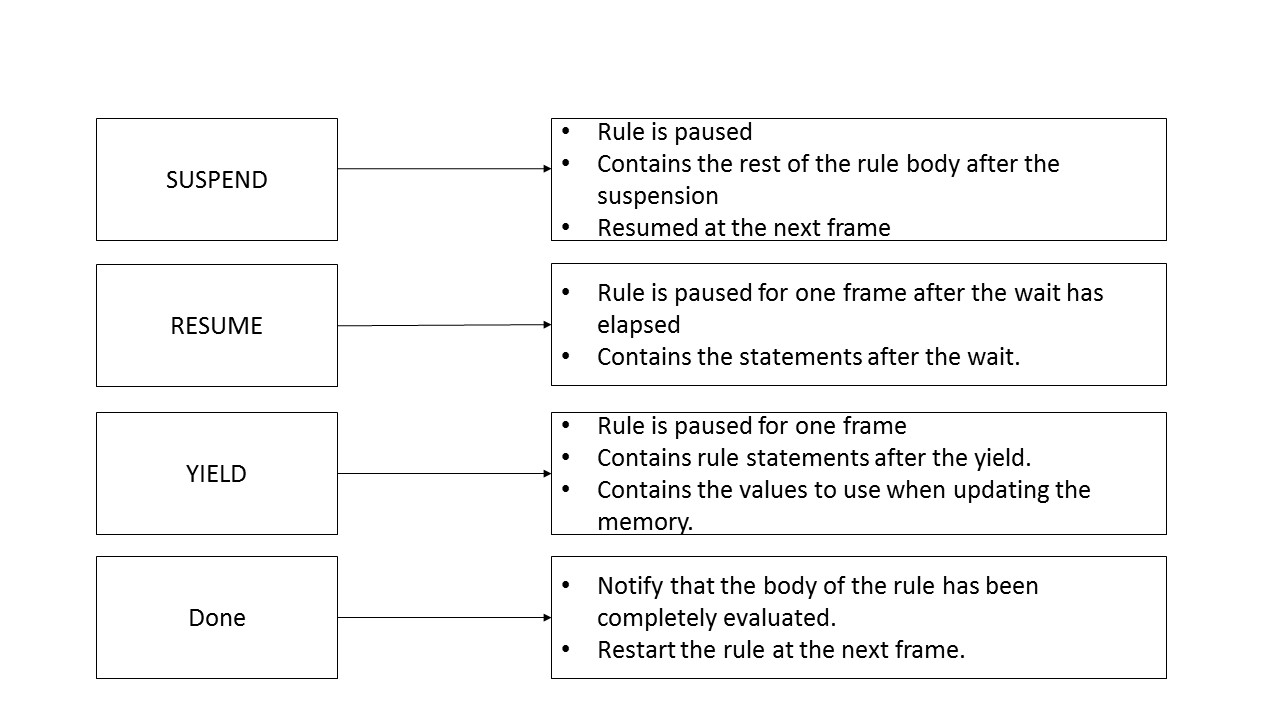
\includegraphics[scale = 0.25]{Figures/tick2}
	\caption{Casanova 2.5 rule evaluation}
	\label{fig:tick}
\end{figure}

The function \texttt{evalRule} calls \texttt{evalStatement} to evaluate the first statement in the body of the rule passed as argument. The result of the evaluation of the statement is processed in the following way: (\textit{i}) if the result is \texttt{Done}, \texttt{Suspend} or \texttt{Resume} then it is just returned to the caller function. We omit the code for this case, since it is trivial; (\textit{ii}) if the result is \texttt{Atomic} it means that the evaluated statement was uninterruptible and the remaining statements of the rule must be re-evaluated immediately; (\textit{iii}) if the result is \texttt{Yield} then the fields in the domain are updated recursively in order and then the updated memory is encapsulated in the \texttt{Yield} data structure and passed to the caller function.

\vspace{0.1cm}
\begin{lstlisting}
evalStatement b k ctxt dt => Atomic z c    
evalRule (rule dom z nop c dt) => res
-------------------------------
evalRule (rule dom b k ctxt dt)  => res
\end{lstlisting}

\begin{lstlisting}
evalStatement b k (Context locals fields globals) dt => Yield ks values context
updateFields dom values context  => updatedContext
--------------------------------------------------------
evalRule (rule dom b k locals dt) fields globals => Yield ks values updatedContex
\end{lstlisting}

Note that, in case of a rule containing only atomic statements, we will eventually return \texttt{Done} after having recursively called \texttt{evalStatement} for all the statements, and the rule will be paused for one frame.

\begin{comment}
\begin{figure}
\centering
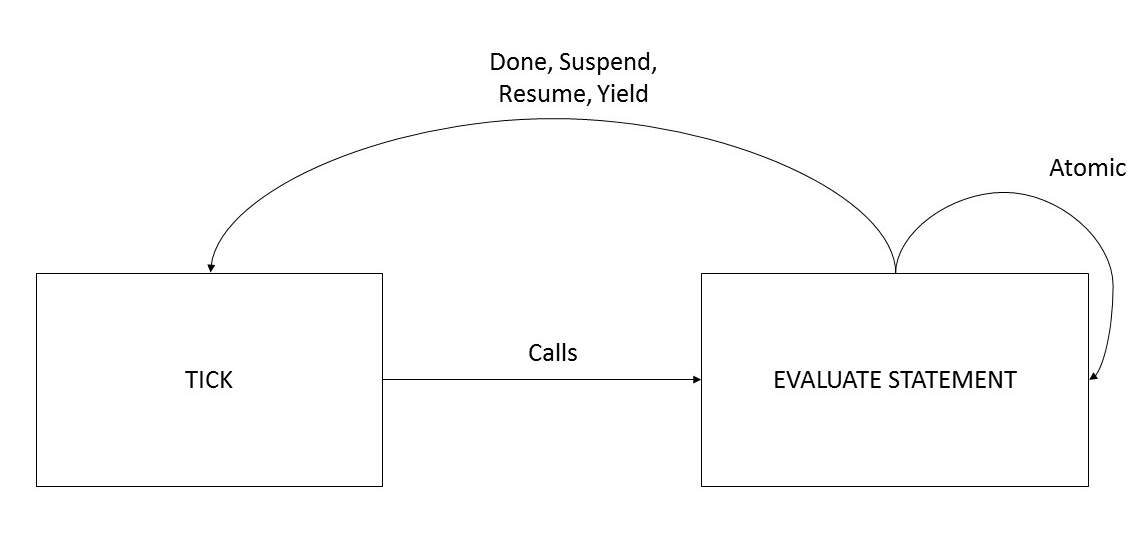
\includegraphics[scale=0.15]{Pictures/statement_evaluation}
\caption{Statement evaluation}
\label{fig:statement_evaluation}
\end{figure}
\end{comment}

\noindent
The \texttt{evalStatement} function is used both to evaluate a single statement and a sequence of statements. When evaluating a sequence of statements, the first one is extracted. A continuation is built with the following statement and passed to a recursive call to \texttt{evalStatement} which evaluates the extracted statement. If the existing continuation is non-empty, then it is added before the current continuation. If both the continuation and the body are empty (situation represented by the \texttt{nop} operator) then it means the rule evaluation has been completed and we return \texttt{Done}.

\begin{lstlisting}
a != nop
---------------------                           ----------------------- 
addStmt a b => a;b                              addStmt nop nop => nop   

addStmt b k => cont
evalStatement a cont ctxt dt => res
-------------------------------                 -----------------------------------       
evalStatement (a;b) k ctxt dt => res            evalStatement nop nop ctxt dt => Done ctxt


\end{lstlisting}

\noindent
We will now present, for brevity, only the evaluation of the \texttt{wait} and \texttt{yield} statements. Both the evaluation of the control structures and the variable bindings always return \texttt{Atomic} because they do not, by definition, pause the execution of the rule.

The \texttt{wait} statement has two different evaluations, based on the rules defined in Section \ref{sec:problem_statement}: (\textit{i}) the timer has elapsed: in this case we return \texttt{Resume} which contains the code to execute after the \texttt{wait} statement, or (\textit{ii}) the timer has not elapsed: in this case we return \texttt{Suspend} which contains the \texttt{wait} statement with the updated timer followed by the continuation.


\begin{lstlisting}
<<t <= dt>> == false
----------------------------------
evalStatement (wait t) k ctxt dt => Suspend wait <<t - dt>>;k ctxt

<<t <= dt>> == true
----------------------------------
evalStatement (wait t) k ctxt dt => Resume k ctxt
\end{lstlisting}

\noindent
The \texttt{yield} statement takes as argument a list of expressions whose values are used to update the corresponding fields in the rule domain. The evaluation rule recursively evaluates the expressions and stores them into a list passed as argument of the \texttt{Yield} result. Those arguments are used later by \texttt{evalRule} to update the corresponding fields.

\begin{lstlisting}
eval expr ctxt => v
evalYield exprs ctxt => vs
-------------------------------------------          ----------------------------
evalYield (expr :: exprs) ctxt => v :: vs            evalYield nil ctxt => nil
\end{lstlisting}

In this section we provide an implementation of a patrol script for an entity in a game. The sample is made up of an entity, representing a guard, and a couple of checkpoints. The guard continuously moves between the two checkpoints. We choose this sample because this is a typical behaviour implemented in several games, where the user is able to set up a patrol route for a unit. We show the comparison between the sample implemented in Casanova 2.5 and an equivalent implementation in Python with respect to the running time. We then show a comparison between the hard-coded compiler of Casanova 2.0 and the implementation of Casanova 2.5 in Metacasanova with respect to the code length. 

\begin{comment}
We want to underline that the main goal of this work is \textbf{to ease the process of building a compiler for a DSL for games, thus our main objective is decreasing the code length and complexity necessary to implement a hard-coded compiler for the language}. At the same time we show that the compiled program in Casanova 2.5 \textbf{has performance similar to that of a language used in game development, and thus Casanova 2.5 is usable in a real scenario}.
\end{comment}

\subsection{Chosen languages}
We compared the running time of the sample in metacompiled Casanova with an equivalent implementation in Python. This language was chosen based on its use in game development: Python has been used extensively in several games such as Civlization IV \cite{CIV4} or World in Conflict \cite{WIC} because of the native support for coroutines. We deliberately ignore C++ and C\# implementations, although they are widely used in the industry, because we knew in advance \cite{CASANOVA2_PAPER} that the current version of the code generated by the meta-compiler would not match the high performance of these languages: the main goal of this work is to reduce the effort of writing a compiler for a DSL for games while having acceptable performance.


\subsection{Performance}
The performance results are shown in Table \ref{tab:evaluation}. We see that the generated code has performance on the same order as Python. This is mainly due to the fact that the memory, in the metacompiled implementation of Casanova, is managed through a map, and because of the virtuality of the implemented operators. Each time Casanova accesses a field in an entity this must be looked up into the map. To this we add the complexity of dynamic lookups when we must deal with polymorphic results into the rules. 

From Table \ref{tab:compiler_comparison} we see that the implementation of Casanova 2.0 language in Metacasanova is almost 5 times shorter in terms of lines of code than the previous Casanova implementation in F\#. We believe it is worthy noticing that structures with complex behaviours, such as \textit{wait} or \textit{when}, require hundreds of lines of codes with a standard approach (the code lines to define the behaviour of the structure plus the support code to correctly generate the state machine), while in the meta-compiler we just need tens of lines of codes to implement the same behaviour. Moreover we want to point out that the previous Casanova compiler was written in a functional programming language: these languages tend to be more synthetic than imperative languages, so the difference with the same compiler implemented in languages such as C/C++ might be even greater.

The readability with respect to the hard-coded compiler code is also improved: we managed to implement the behaviour of synchronization and timing primitives almost imitating one to one the formal semantics of the language definition (see the semantics rules in Section \ref{sec:formal_description} and their implementation in Section \ref{sec:casanova3}). In the hard-coded compiler implementation for Casanova 2.0 the semantics are lost in the code for generating finite state machines.

\begin{table}[!h]
	\centering
	\tiny	
	\begin{tabular}{|c|c|c|}
		\hline
		\multicolumn{3}{|c|}{\textbf{Casanova 2.5}} \\
		\hline
		Entity \# & Average update time (ms) & Frame rate \\
		\hline
		100 & 0.00349 & 286.53 \\
		\hline
		250 & 0.00911 & 109.77 \\
		\hline
		500 & 0.01716 & 58.275 \\
		\hline
		750 & 0.02597 & 38.506 \\
		\hline
		1000 & 0.03527 & 28.353 \\
		\hline
		\multicolumn{3}{|c|}{\textbf{Python}} \\
		\hline
		Entity \# & Average update time (ms) & Frame rate \\
		\hline
		100 & 0.00132 & 756.37 \\
		\hline
		250 & 0.00342 & 292.05 \\
		\hline
		500 & 0.00678 & 147.54 \\
		\hline
		750 & 0.01087 & 91.988 \\
		\hline
		1000 & 0.01408 & 71.002 \\
		\hline
	\end{tabular}
	\caption{Patrol sample evaluation}
	\label{tab:evaluation}
\end{table}

\begin{table}[!h]
	\centering
	\tiny
	\begin{tabular}{|c|c|}
		\hline
		\multicolumn{2}{|c|}{\textbf{Casanova 2.5 with Metacasanova}} \\
		\hline
		Module & Code lines \\
		\hline
		Data structures and function definitions & 40 \\
		\hline
		Query Evaluation & 16 \\
		\hline
		While loop & 4 \\
		\hline
		For loop & 5 \\
		\hline
		If-then-else & 4 \\
		\hline
		When & 4 \\
		\hline
		Wait & 6 \\
		\hline
		Yield & 10 \\
		\hline
		Additional rules for Casanova program evaluation & 40 \\
		\hline
		Additional rules for basic expression evaluation & 201 \\
		\hline
		\multicolumn{2}{|l|}{\textbf{Total: } 300} \\
		\hline
		\multicolumn{2}{|c|}{\textbf{Casanova 2.0 compiler}} \\
		\hline
		Module & Code lines \\
		\hline
		While loop & 10 \\
		\hline
		For-loop and query evaluation & 44 \\
		\hline
		If-Then-Else & 15 \\
		\hline
		When & 11 \\
		\hline
		Wait & 24 \\
		\hline
		Yield & 29 \\
		\hline
		Additional structures for rule evaluation & 63 \\
		\hline
		Structures for state machine generations & 754 \\
		\hline
		Code generation & 530 \\
		\hline
		\multicolumn{2}{|l|}{\textbf{Total: } 1480} \\
		\hline			
	\end{tabular}	
	\caption{meta-compiler vs standard compiler}
	\label{tab:compiler_comparison}
\end{table}

\subsection{Discussion}
\label{subsec:code_generation_discussion}
Metacasanova has been evaluated in \cite{DiGiacomo2017} by re-building the DSL for game development Casanova \cite{abbadi2015casanova, abbadithesis2017}. Even though the size of the code required to implement the language has been drastically reduced (almost 1/5 shorter), performance dropped dramatically. We identified a main problem causing the performance decay that, if solved, will improve the performance of the generated code.

In order to encode a symbol table in the meta-compiler in the current implementation (used for example to store the variables defined in the local scope of a control structure or to model a class/record data structure), we are left with two options: (\textit{i}) define a custom data structure made of a list of pairs, containing the field/variable name as a string and its value, in the following way

\begin{lstlisting}
Data "table" -> List[Tuple[string, Value]] : SymbolTable
\end{lstlisting}

\noindent
or (\textit{ii}) use a dictionary data structure coming from .NET, such as \texttt{ImmutableDictionary}, which was the implementation choice for Casanova. In both cases, the behaviour of the language implemented in Metacasanova will be that of a dynamic language, because whenever the value of a variable or class field must be read, the evaluation rule must look up the symbol table at run time to retrieve the value, whose complexity will be $O(n)$ with the list implementation and $O(\log n)$ with the dictionary implementation. This issue is caused by the fact that, in the current state of Metacasanova, the meta-type system is unaware of the type system of the language that is being implemented in the meta-compiler. This is not a problem limited to Metacasanova but to all meta-compilers having a meta-type system that does not allow embedding of the host language type system. In the next section we propose an extension to Metacasanova to overcome this problem by embedding the type system of the implemented language in the meta-type system of Metacasanova and inlining the code to access the appropriate variable at compile time.


